\section{Experimental Setup}\label{sec:experimental-setup}

Length: 1-2 pages

Explain the overall design of the complete system and list the
configurations (number of middlewares, number of clients, types of
machines, communication patterns) corresponding to the main workloads.

Describe the mechanisms for deploying the system for experiments and the
way performance numbers are gathered and processed. Make the description
so that someone unfamiliar with your system can replicate the steps, and
reference the different script files you submit as code in the SVN
repository.

\subsection{System Configurations}\label{sec:system-configurations}
.	Overall there are three tier components in the system, as it was described in the requirements. The tiers are the database machine, two middleware machines and two client machines. All the machines are t2.medium Amazon EC2 instances. In order to build the Middleware and Client applications Ant was used.
\subsection{Configuration and Deployment mechanisms}\label{sec:configuration-and-deployment-mechanisms}
For configuration of each client as mention in 2.1 the Middleware and the Client were built using Ant. In order to deploy the system including the Database and applications in each tier Python scripts were used. A main script with different function was written in order to perform different operations within the system. Moreover, fabric a python library that works as command line tool and ssh application was used as part of the deployment process.
\subsection{Logging and Benchmarking mechanisms}\label{sec:logging-and-benchmarking-mechanisms}
\begin{figure}[h!]
	\centering
	%\def \svgscale {\columnwidt}
	
\includegraphics[scale=0.3]{logging.png}
	\caption{Different logging entry point during the lifespan of a single request in the messaging system}
	\label{logging}
	%\input{soft-mmu-2.pdf}
\end{figure}
 For the logging mechanism the library lo4j was used. The configuration files is passed as parameter to the Clients and the Middleware application. Both components log the type of request they are preforming, with a timestamp and the number of the request.\\
 
The client just before sending the request make a log entrance and once it get the response enters a second log. In the middleware a log entrance is made when the Middleware gets the request from the client, then when it sends a request to the database and when the request return from it, this one is to estimate the response time of the database from the middleware perspective. Finally after sending the response to the client it enters another log entrance. See Figure \ref{logging}.\\

Finally for benchmarking a python method is the tool is script was written in order to parse the result of the logs provided the middleware and the clients. In addition the middleware has embedded another logging functions to log the throughput of the middleware every second during the execution of it. With those numbers in the log files and the parsing method numbers of the performance of the system were gathered.

\section{Evaluation}\label{sec:evaluation}


\subsection{System Stability}\label{sec:system-stability}

\begin{figure}[h!]
	\centering
	%\def \svgscale {\columnwidt}
	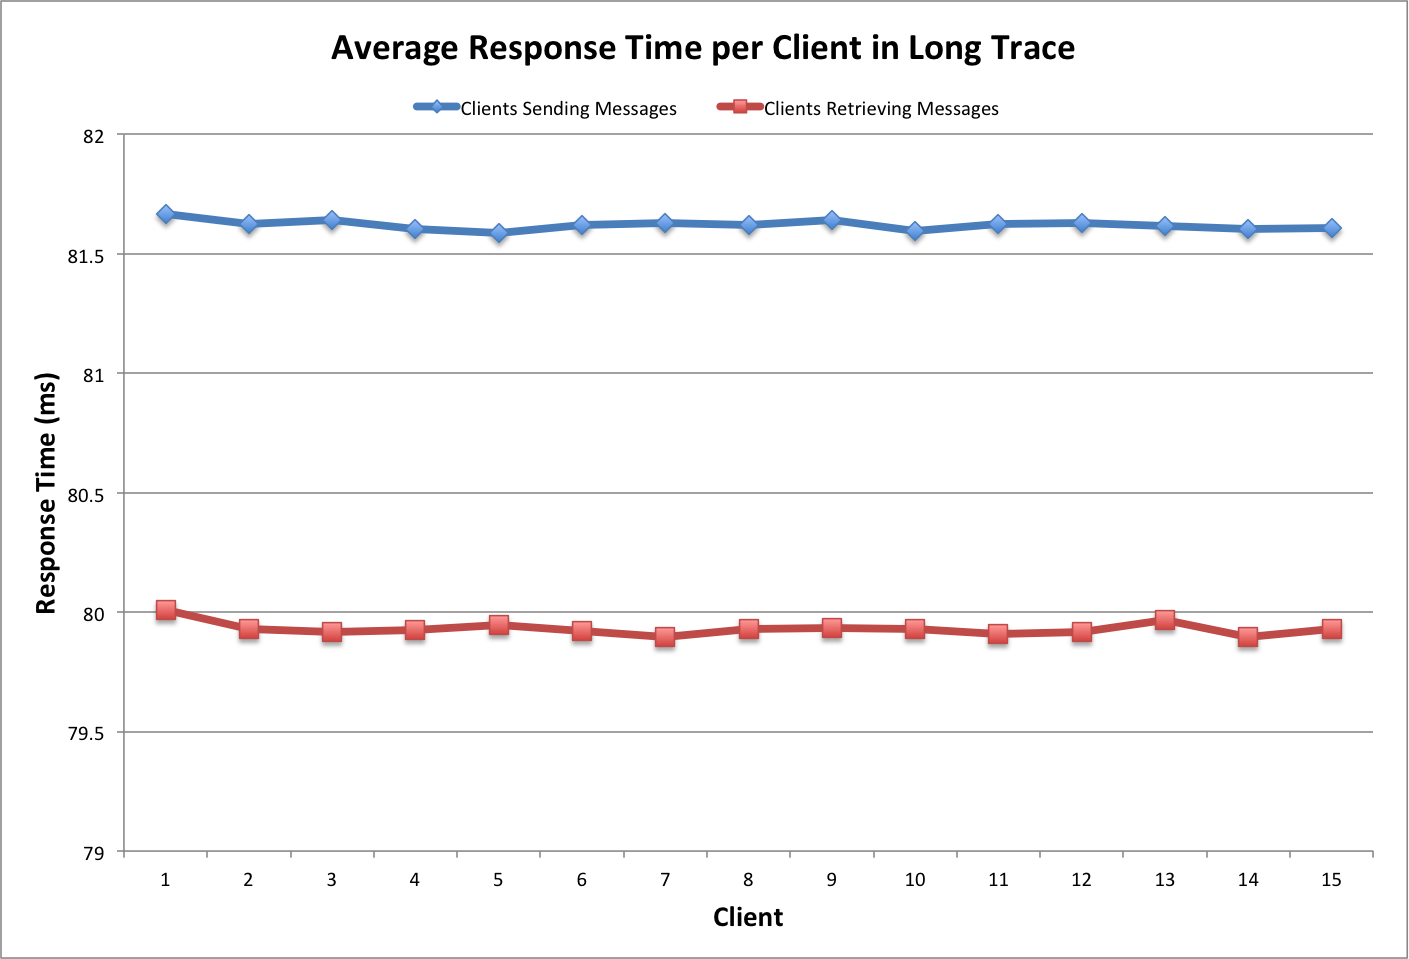
\includegraphics[scale=0.35]{stabilityRP.png}
	\caption{}
	\label{stabilityRP}
	%\input{soft-mmu-2.pdf}
\end{figure}
\begin{figure}[h!]
	\centering
	%\def \svgscale {\columnwidt}
	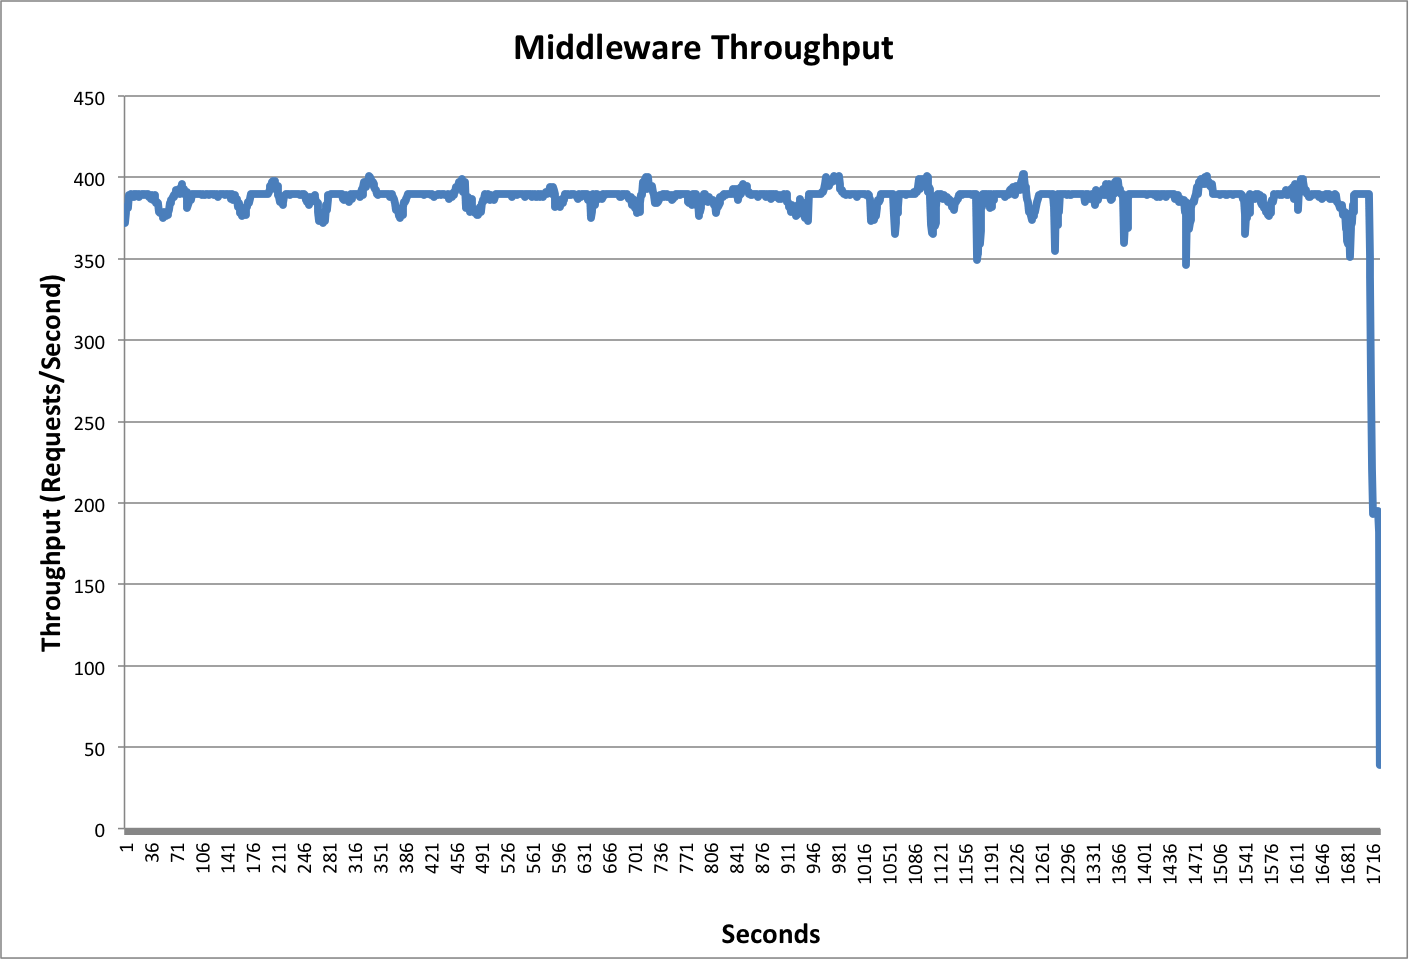
\includegraphics[scale=0.45]{stabilityTHR.png}
	\caption{}
	\label{stabilityTHR}
	%\input{soft-mmu-2.pdf}
\end{figure}
\subsection{System Throughput}\label{sec:system-throughput}

Measure the maximum throughput of the system (describe the exact
configuration and workload, and the reasoning behind choosing these
particular ones) and show the average response time for this experiment.

\subsection{System Scalability}\label{sec:system-scalability}

Explain the different configurations used to explore the scalability of
your system, and the outcomes of these experiments in terms of
throughput and response times. The main goal of this subsection is to
define the ranges in which your system operates best.

\subsection{Response Time Variations}\label{sec:response-time-variations}

Report and analyze how the response times change in the system with
different message sizes, different number of clients and different
number of middleware nodes.

\subsection{$2^k$ Experiment}\label{sec:k-experiment}

Conduct a 2\^{}k analysis of your system (aim at exploring non-obvious
interactions of parameters). Use the methods learned in this lecture to
conduct the detailed analysis.

\subsection{Conclusion}\label{sec:conclusion}

To conclude the report summarize the behavior of the system in terms of
the design and the representative workloads. Finally, outline in a few
points what would you do differently if you could design the system
anew.